\tikzstyle{component} = [draw, text width=4em, fill=gray!10, text centered,
    minimum height=8em, rounded corners]
\def\arrdist{1.5em}

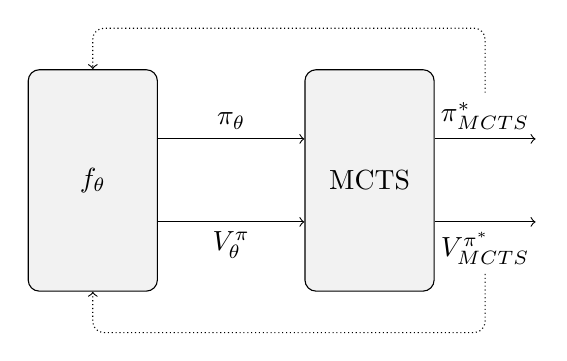
\begin{tikzpicture}
    \node (mcts) [component] {MCTS};
    \node (neural_net) [component, xshift=-10em] {$f_\theta$};
    
    \draw[->] ([yshift=\arrdist]neural_net.east) -- node [above] {$\pi_\theta$} ([yshift=\arrdist]mcts.west);
    \draw[->] ([yshift=-\arrdist]neural_net.east) -- node[below] {$V^\pi_\theta$} ([yshift=-\arrdist]mcts.west);

    \path [draw, ->] ([yshift=-\arrdist]mcts.east) -- node[below] (mcts_v) {$V^{\pi^*}_{MCTS}$} ([yshift=-\arrdist]6em, 0);
    \path [draw, ->] ([yshift=\arrdist]mcts.east) -- node[above] (mcts_pi) {$\pi^{*}_{MCTS}$} ([yshift=\arrdist]6em, 0);

    \path [draw, ->, densely dotted, rounded corners] (mcts_pi.north) |- (0, 5.5em) -| (neural_net.north);
    \path [draw, ->, densely dotted, rounded corners] (mcts_v.south) |- (0, -5.5em) -| (neural_net.south);
\end{tikzpicture}